%!TEX root = ../book.tex
\chapter{Locomotion, manipulation and their representations}\label{chap:locomotion}

Autonomous robots are systems that sense, compute, communicate, and actuate. Actuation, the focus of this chapter, is the ability of the robot to move and to manipulate the world. Specifically, we differentiate between locomotion\index{Locomotion} as the robot's ability to move itself and manipulation\index{Manipulation} as the robot's ability to move objects in the environment. Both activities are closely related: during locomotion the robot uses its motors to exert forces on its environment (ground, water, or air) to move itself; during manipulation it uses motors to exert forces on objects to move them relative to the rest of the environment. This might not even require different motors. Insects are good examples for this: they can use their six legs not only for locomotion, but also for picking up and manipulating objects. In short, the goals of this chapter are to:
\begin{itemize}
\item Introduce the concepts of locomotion, manipulation and their duality,
\item Explain static vs.\ dynamic stability,
\item Introduce the concept of ``Degree of Freedom'' (DoF),
\item introduce coordinate systems and their transformations.
\end{itemize}

\section{Locomotion and manipulation examples}

Locomotion includes very different concepts of motion, including rolling, walking, running, jumping, sliding (undulatory locomotion), crawling, climbing, swimming, and flying. The mechanisms that might achieve these feats could be drastically different in terms of energy consumption, kinematics, stability, and other capabilities required by the robot that implements them. Furthermore, the above definitions are loose and ambiguous: for example, ``swimming'' can be performed using many different forms of propulsion. Similarly, a sliding motion on the ground might work well for swimming too with only few modifications.

The way in which the individual parts of a robot can move with respect to each other and the environment is called the \textsl{kinematics}\index{Kinematics} of the robot. Kinematics (which will be discussed in detail in \cref{chap:kinematics}) are only concerned with the position and speed (first derivative of position) of those parts; depending on the application, one may want to use a deeper level of abstraction called \textsl{dynamics}\index{Dynamics}, which is concerned with quantities such as acceleration (second derivative of position) and jerk (third derivative of position).

Commercially, the most widespread form of locomotion is rolling. This is partially due to the fact that rolling provides by far the most efficient energy to speed ratio (see \cref{fig:todd}), making the invention of the wheel one of the greatest technological breakthroughs in history. It also is a widely implemented form of locomotion, e.g.\ with cars and bicycles. Consequently, humans have modified their environment to have as many smooth surfaces as possible---e.g. roads, warehouses, and residential floors.
%
In contrast, evolution has not equipped any animal with wheel-like actuators because of their poor performance in natural environments such as an unmown meadow, a forest floor, a mountains or a cave; consequently, wheeled robots perform poorly in such environments, whereas legged robots can shine.

\begin{figure}
    \centering
    \includegraphics[width=0.8\textwidth]{figs/todd85.png}
    \caption{Power consumption vs.\ speed for various means of locomotion. From \protect\citeasnoun{todd1985walking}.}
    \label{fig:todd}
\end{figure}


\begin{mdframed}Can you find examples of robots from the above categories (legged vs wheeled robots)? Identify the different types of actuators that are used in them.
\end{mdframed}

Most mechanisms capable of locomotion can also be used for manipulation with only minor modifications. Most industrial manipulators consist of a chain of rotary (or revolute) actuators that are connected by rigid links. In general, they are equipped with six or more independently rotating axes---we will see why further down below. In addition, modern industrial manipulators have the ability to not only control the position of each of its joints, but to also control the torque at each individual joint; this capability allows control over the \textsl{compliance}\index{Compliance} of a robot, which in a mechanical sense is the inverse of stiffness. Finally, for dexterous manipulation a robot does not only need an arm, but also a gripper or hand. Grasping is a hard problem on its own and is therefore treated in its own chapter (\cref{chap:grasping}).


Regardless of whether the robot is rolling or walking, the dominant actuator type is rotational. Another type of mechanism is the \emph{prismatic} or \emph{linear} joint (see Figure \ref{fig:prismaticjointkinematics} for example) that allows the robot to extend and contract a link. This type of joints are usually combined with rotating joints and allow, for example, a robot arm to move up and down, or a robotic walker to extend or retract its leg. 

%This lecture focuses on the kinematics of simple mechanisms. Understanding the duality between locomotion and manipulation is important, however, to better introduce (and understand) concepts such as reference frames and forward kinematics.

\section{Static and dynamic stability}\label{sec:stability}

A fundamental difference between locomotion mechanisms is whether they are statically or dynamically stable\index{Static stability}\index{Dynamic Stability}. A statically stable mechanism will not fall even when not actuated (\cref{fig:stability}, left). A dynamically stable robot instead requires constant actuation to prevent it from falling. Technically, stability requires the robot to keep its center of mass to fall within the polygon spanned by its ground-contact points. For example, a quadrupedal robot's feet span a rectangle. Once such a robot lifts one of its feet, this rectangle becomes a triangle. If the projection of the center of mass of the robot along the direction of gravity is outside of this triangle, the robot will fall. A dynamically stable robot can overcome this problem by changing its configuration so rapidly that a fall is prevented. An example of a purely dynamically stable robot is an inverted pendulum on a cart (\cref{fig:stability}, middle). Such a robot has no statically stable configurations and needs to keep moving all the time to keep the pendulum upright. While dynamic stability is desirable for high-speed, agile motions, robots should be designed so that they can easily switch into a statically stable configuration (\cref{fig:stability}, right).

\begin{figure}
    \centering
    % 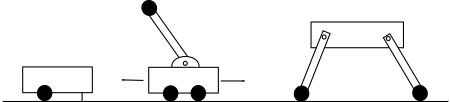
\includegraphics[width=\textwidth]{figs/stability.png}
    \def\svgwidth{\textwidth}
    \import{./figs/}{stability.pdf_tex}
    \caption{From left to right: statically stable robot; dynamically stable inverted pendulum robot; static and dynamically stable robot (depending on configuration).}
    \label{fig:stability}
\end{figure}

An example of a robot that has both statically and dynamically stable configurations is a quadruped running. Unlike walking, a running quadruped robot will always have two legs in the air and alternate between them faster than the robot may fall in either direction. Although statically stable walking is possible with only four legs, most animals (and robots) require six legs for statically stable walking and use dynamically stable gaits (such as galloping) when they have four legs. Six legs allow the animal to move three legs at a time while the three other legs maintain a stable pose.


\section{Degrees of freedom}\label{sec:dof}

The concept of \textsl{degree of freedom}\index{Degree of Freedom}, often abbreviated as DoF, is important for defining the possible positions and orientations a robot can reach. An object in the physical world can have up to six \textsl{Cartesian}\index{Cartesian}\index{Cartesian Degree of Freedom} degrees of freedom, namely forward/backward, sideways, and up/down as well as rotations around those axes. These rotations are known as pitch, yaw, and roll and are illustrated in \cref{fig:pitchyawandroll}. These Cartesian degrees of freedom are distinct from the robot's \textsl{mechanical} degrees of freedom, which correspond to the number of points of actuation for a robot (i.e., a robotic arm with five joint motors is referred to as having five mechanical degrees of freedom \textsl{in joint space}, see \cref{chap:kinematics}).
As a rule of thumb, the number of mechanical DoFs available to the user depends on the robot platform and cannot easily be changed by the user unless mechanical modifications to the robot are made; conversely, the number of Cartesian DoFs depends on the task, can be modified by the user, and varies according to what the robot needs to do.

\begin{figure}
    \centering
    % 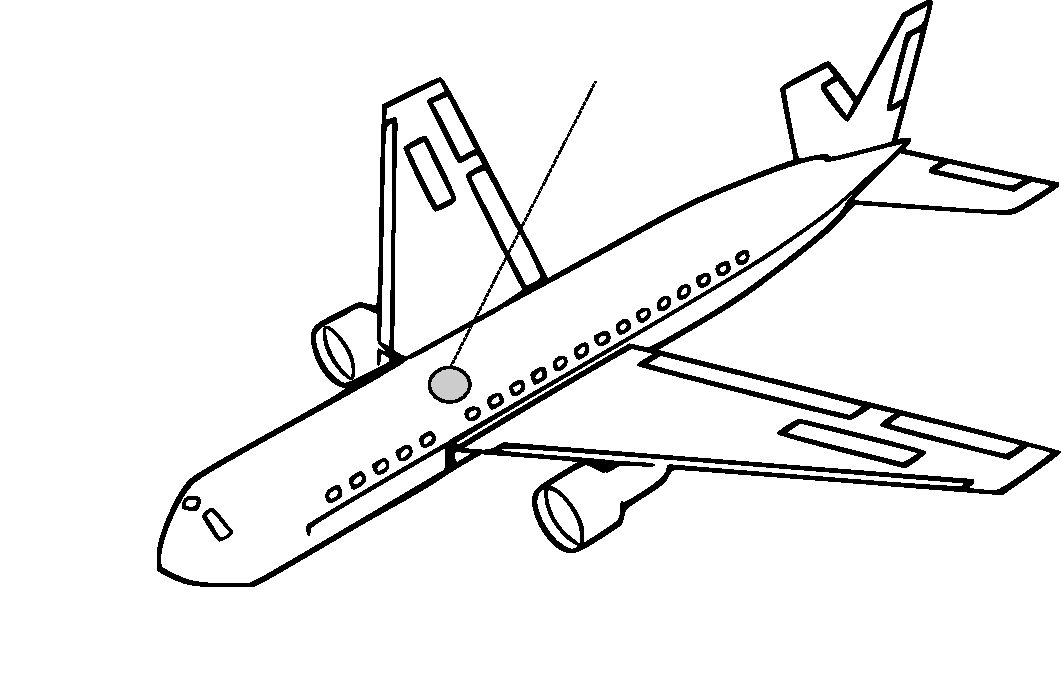
\includegraphics[width=\textwidth]{figs/pitchyawroll.png}
    \def\svgwidth{\textwidth}
    \import{./figs/}{pitchyawroll.pdf_tex}
    \caption{Pitch, yaw, and roll around the principal axis of an airplane.}
    \label{fig:pitchyawandroll}
\end{figure}

After specifying the mechanical and Cartesian DoFs for your kinematic problem, the number of Cartesian DoFs (i.e. directions) a robot can actually move in depends on the configuration of its actuators and the constraints the robot has with the environment. These relationships are not always intuitive and require more rigorous mathematical treatment (see \cref{chap:kinematics}). The goal of this section is to introduce the degrees of freedom of standard mechanisms that are recurrent in robot design such as wheels or simple arms. For wheeled platforms, the degrees-of-freedom are defined by the types of wheels used and their orientation. Common wheel types are listed in \cref{tab:wheels}.

\begin{table}\centering
\begin{tabular}{p{2.5cm}p{2.6cm}p{4.7cm}}
\hline
Wheel type & Example & Degrees of Freedom\\
\hline
Standard
% 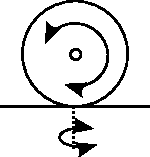
\includegraphics[width=2.5cm]{figs/wheeltype_standard.png}
\def\svgwidth{2.5cm}
\import{./figs/}{wheeltype_standard.pdf_tex}  & Front-wheel of a wheelbarrow    & Two:%
\begin{itemize}[wide=0.8\parindent,listparindent=4pt,itemsep=-2pt]
\item Rotation around the wheel axle
\item Rotation around its contact point with the ground
\end{itemize}\\
\hline
Caster wheel
% 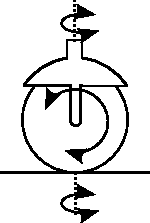
\includegraphics[width=2.5cm]{figs/wheeltype_caster.png}
\def\svgwidth{2.5cm}
\import{./figs/}{wheeltype_caster.pdf_tex}  & Office chair & Three:%
\begin{itemize}[wide=0.8\parindent,listparindent=4pt,itemsep=-2pt]
\item Rotation around the wheel axle
\item Rotation around its contact point with the ground
\item Rotation around the caster axis
\end{itemize}\\
\hline
Swedish wheel
% 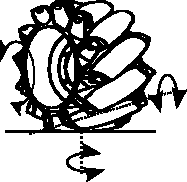
\includegraphics[width=2.5cm]{figs/wheeltype_swedish.png}
\def\svgwidth{2.5cm}
\import{./figs/}{wheeltype_swedish.pdf_tex} & Standard wheel with non-actuated rollers around its circumference& Three:%
\begin{itemize}[wide=0.8\parindent,listparindent=4pt,itemsep=-2pt]
\item Rotation around the wheel axle
\item Rotation around its contact point with the ground
\item Rotation around the roller axles
\end{itemize}\\
\hline
Spherical wheel
% 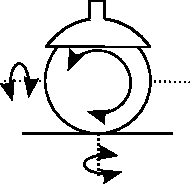
\includegraphics[width=2.5cm]{figs/wheeltype_spherical.png}
\def\svgwidth{2.5cm}
\import{./figs/}{wheeltype_spherical.pdf_tex} & Ball Bearing & Three:%
\begin{itemize}[wide=0.8\parindent,listparindent=4pt,itemsep=-2pt]
\item Rotation in any direction
\item Rotation around its contact point
\end{itemize}\\
\hline
\end{tabular}
\caption{Different types of wheels and their degrees of freedom. Adopted from \protect\citeasnoun{siegwart2011introduction}.}\label{tab:wheels}
\end{table}

Only robots that use exclusively use wheels with three degrees-of-freedom ($3$-DoF wheels) will be able to freely move on a plane. This is because the pose of a robot on a plane is fully determined by its position (two values, e.g. vertical and horizontal position) and its orientation (one value, e.g. an angle). Robots that don't have wheels with three degrees of freedom will have \textsl{kinematic constraints}\index{Kinematic constraints} that prevent them from reaching every possible point at every possible orientation. For example, a bicycle wheel can only roll along one direction and turn on the spot. Moving the bicycle wheel orthogonally to its direction of motion is not possible, unless it is forcefully dragged (``skidding''). Importantly, not having three degrees of freedom does not imply that some poses in the plane are unreachable---it may just require additional movements to achieve them!

A good analogue are figures on a chess-board. For example, a knight can reach every cell on a chess-board but might require multiple moves to do so. This is similar to a car, which can parallel park using back-and-forth motions. Instead, a bishop can only reach either black or white fields on the board, based upon its starting position.

Similar reasoning applies to aerial and underwater robots. Here, the position of the robot is affected by the position and orientation of its thrusters, either in the form of jets or propellers. Things become complicated quickly, however, as the dynamics of the system are subject to fluid-dynamic and aero-dynamic effects, which also change as a function of the size of the robot. This book will not go into the details of flying and swimming robots, but the general principles of localization and planning will be applicable to them as well.

\begin{mdframed} Think about possible wheel, propeller and thruster configurations. Don't limit yourself to robots, but consider also street and aerial vehicles and be creative---if you can think about a setup that makes sense, i.e., allows for reasonable mobility---somebody has already built it and analyzed it. What are the advantages and disadvantages of each?
\end{mdframed}

For manipulating arms, Cartesian DoFs refer to the positions and orientations (rotations around the primary axes ($x$, $y$, and $z$) that the end-effector can reach. Each actuated joint will typically add a degree of freedom, unless it is redundant (moving in the same direction, with the same physical effect, as a different joint). \cref{fig:basickinematics,fig:prismaticjointkinematics} show a series of manipulators operating on a planar surface. In such a scenario, the degrees of freedom of the end-effector are limited to moving up and down, sideways, and rotating around their pivot point. As a plane only has those three degrees of freedom, adding additional joints will not increase the number of Cartesian DoFs unless they allow the robot to also move in and out of the plane (``vertical'' axis).
%
An exact definition of the number of degrees of freedom is tricky and requires deriving analytical expressions for the end-effector position and orientation, which will be the subject of \cref{chap:kinematics}.

\begin{figure}[!htb]
    \centering
    % 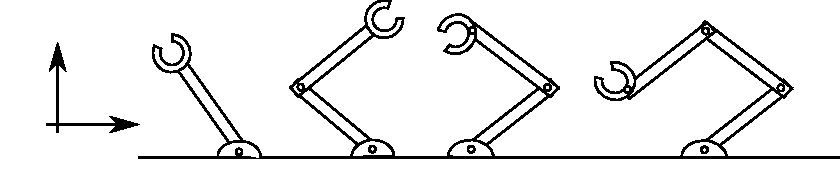
\includegraphics[width=\textwidth]{figs/basickinematics.png}
    \def\svgwidth{\textwidth}
    \import{./figs/}{basickinematics.pdf_tex}
    \caption{From left to right: Manipulators with one, two, three and four mechanical DoFs. The Cartesian DoFs needed for the end-effector to move in a plane are: the vertical displacement of the end-effector with respect to the base, its horizontal displacement, and its orientation.}
    \label{fig:basickinematics}
\end{figure}

\begin{figure}[!htb]
    \centering
    % 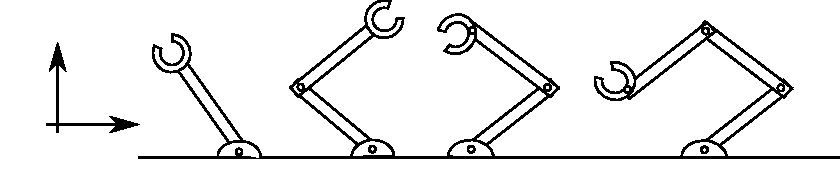
\includegraphics[width=\textwidth]{figs/basickinematics.png}
    \def\svgwidth{\textwidth}
    \import{./figs/}{prismaticjointkinematics.pdf_tex}
    \caption{From left to right: Manipulators with one, two, three, and four DoFs using a combination of rotational and prismatic joints.}
    \label{fig:prismaticjointkinematics}
\end{figure}

Choosing the ``right'' kinematics involves a very complex trade-off between mechanical complexity, maneuverability, achievable precision, cost, and ease of control. The very popular differential-wheel drive---consisting of two independently controlled wheels that share a common axis, such as those mounted on a robotic vacuum cleaner---is cheap, highly maneuverable, and easy to control; however, it is hard to drive the robot in a perfectly straight line. This motion requires both motors to turn at the exact same speed and both wheels to have the exact same diameter, which is hard to achieve in practice. This problem is solved well by car-like steering mechanisms---which in turn have poor maneuverability and are difficult to control (as a reference, think about the complexity of parallel parking).

\section{Coordinate Systems and Frames of Reference}\label{sec:coordsystems}

\screencast{http://youtu.be/klBJi-MEeNQ}{coordinatesystem}

Every robot assumes a position in the real world that can be described by its position (x, y and z) and orientation (pitch, yaw and roll) along the three major axes of a Cartesian Coordinate system (see also \cref{sec:dof}).
Such a coordinate system is shown in \cref{fig:coordinatesystem}. Note that the directions and orientations of the coordinate axes are arbitrary. This book uses the ``right hand rule'', which is illustrated in \cref{fig:coordinatesystem} to determine axes labels and directions throughout.
Pitch, yaw, and roll, are also known as bank, attitude, and heading in other communities\index{Pitch}\index{Yaw}\index{Roll}\index{Bank}\index{Attitude}\index{Heading}. This makes sense, considering the colloquial use of the word ``heading'', which corresponds to a rotation around the z-axis of a vehicle driving on the x-y-plane.

\begin{figure}
    \centering
    % 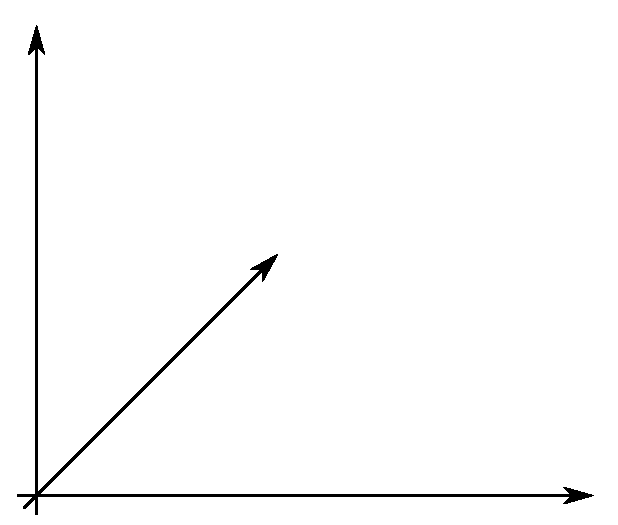
\includegraphics[width=0.8\textwidth]{figs/coordinatesystem}
    \def\svgwidth{0.8\textwidth}
    \import{./figs/}{coordinatesystem.pdf_tex}
    \caption{A coordinate system indicating the direction of the coordinate axes and rotation around them. These directions have been derived using the right-hand rules.}
    \label{fig:coordinatesystem}
\end{figure}

Defining all three position axes and orientations might be cumbersome. What level of detail we care about, where the origin of this coordinate system is, and even what kind of coordinate system we choose, depends on the specific application.
For example, a simple mobile robot would typically require a representation with respect to a room, a building, or the earth's coordinate system (given by the longitude and latitude of each point on earth), whereas a static manipulator usually has the origin of its coordinate system at its base.
More complicated systems, such as mobile manipulators or multi-legged robots, make life much easier by defining multiple coordinate systems, e.g.\ one for each leg and one that describes the position of the robot in the world frame. These local coordinate systems are known as \emph{Frames of Reference}\index{Frame of Reference}.
An example of two nested coordinate systems is shown in \cref{fig:nestedcoords}. In this example, a robot located at the origin of $x',y'$ and $z'$ might plan its motions in its own reference frame, which can then be expressed in the coordinate system $x$, $y$ and $z$ by performing a translation and a rotation---as we will later see.

Depending on its degrees of freedom in Cartesian space---that is, the number of independent translations and rotations a robot can achieve in such a space---it is also customary to ignore components of position and orientation that remain constant.
For example, a simple floor-cleaning robot's pose might be completely defined by its $x$ and $y$ coordinates in a room as well as its orientation, i.e.\ its rotation around the $z$-axis. In this case, $z$ position and rotation around $x$ and $y$ axes would be ignored.

\begin{figure}
    \centering
    %
\includegraphics[width=\textwidth]{figs/frameofreference.png}
    \def\svgwidth{\textwidth}
    \import{./figs/}{nestedcoords.pdf_tex}
    \caption{Two nested coordinate systems (also referred to as frames of reference).}
    \label{fig:nestedcoords}
\end{figure}

\subsection{Matrix notation}
Given some kind of fixed coordinate system, we can describe the \emph{position} of a robot's end-effector by a $3\times1$ position vector.
As there can be many coordinate systems defined on a robot and the environment, we identify the coordinate system a point relates to by a preceeding super-script, e.g., $ ^AP$ to indicate that point $P$ is in coordinate system $\{A\}$.
Each point consists of three elements $ ^AP=[p_x, p_y, p_z]^T$.

More formally, $^AP$ is a linear combination of the three basis vectors that span $A$:
\begin{equation}
^AP=p_x\left[\begin{array}{c}1\\0\\0\end{array}\right]+p_y\left[\begin{array}{c}0\\1\\0\end{array}\right]+p_z\left[\begin{array}{c}0\\0\\1\end{array}\right]\label{eq:basis}
\end{equation}

\screencast{http://youtu.be/QdHO_9M8-UI}{frameofreference}

As we know, not only the position of the robot is important, but also its orientation.
In order to describe the orientation of a point, we will attach a coordinate system to it. Let $ \hat{X}_B, \hat{Y}_B$ and $ \hat{Z}_B$ be unit vectors that correspond to the principal axes of a coordinate system $\{B\}$.
When expressed in coordinate system $\{A\}$, they are denoted $^A\hat{X}_B, ^A\hat{Y}_B$ and $ ^A\hat{Z}_B$.
In order to express a vector that is given in one coordinate system in another, we need to \textsl{project} each of its components to the unit vectors that span the target coordinate system. For example, if we consider only the axis $^A\hat{X}_B$, we have that:

\begin{equation}\label{eq:projection}
^A\hat{X}_B=(\hat{X}_B\cdot\hat{X}_A, \hat{X}_B\cdot\hat{Y}_A,\hat{X}_B\cdot\hat{Z}_A)^T
\end{equation}

consists of the projections of $\hat{X}_B$ onto $\hat{X}_A$, $\hat{Y}_A$ and $\hat{Z}_A$. Here, `$\cdot$' denotes the scalar product (also known as dot or inner product, see \cref{app:linalg:dotproduct}).
Note that all vectors in (\ref{eq:projection}) are unit vectors, i.e.\ their length is one.
By following the definition of the scalar product, we have that $A\cdot B=\|A\|\|B\|\cos \alpha=\cos \alpha$, indeed reduces the projection of $\hat{X}_B$ onto the unit vectors of $\{A\}$. This projection is illustrated in \cref{fig:projection}.

\begin{figure}
    \centering
    % 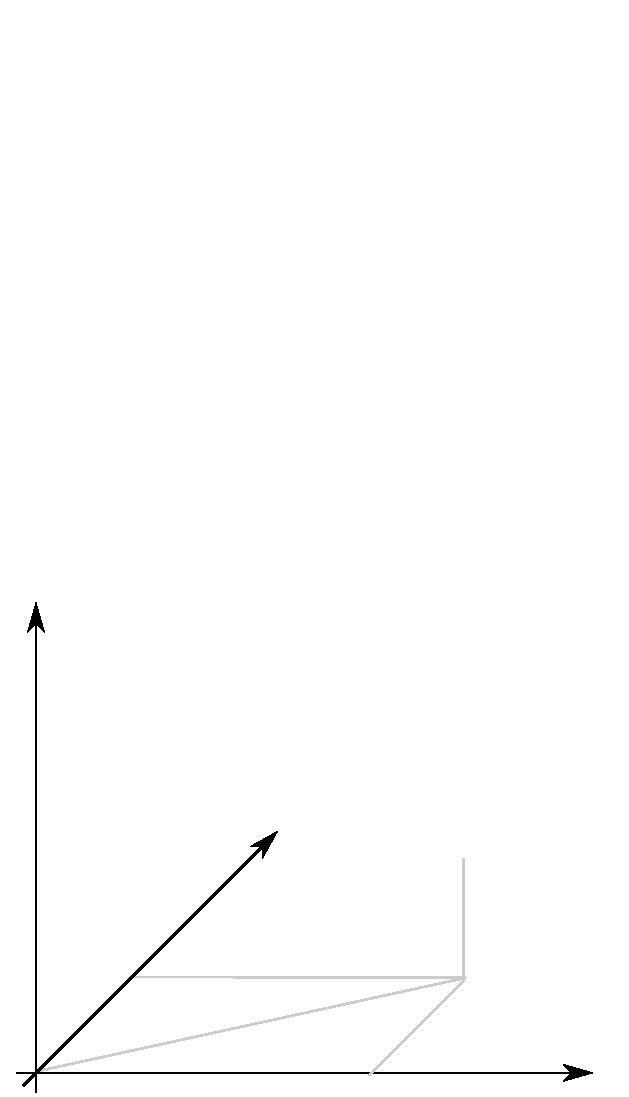
\includegraphics[width=0.8\textwidth]{figs/projection.png}
    \def\svgwidth{0.8\textwidth}
    \import{./figs/}{projection.pdf_tex}
    \caption{Top: A coordinate system $\{B\}$ with position given by $^AP$ and orientation given by $\hat{X}_B$, $\hat{Y}_B$, and $\hat{Z}_B$. Bottom:
    The projection of the unit vector $\hat{X}_B$ onto the unit vectors that span coordinate system $\{A\}$ after moving $\{B\}$ into the origin of $\{A\}$. As all vectors are unit vectors, $A\cdot B=\|A\|\|B\|\cos \alpha=\cos \alpha$. }
    \label{fig:projection}
\end{figure}

We can now apply the same procedure to all three vectors that span coordinate system $\{B\}$ and stack these three vectors together into a $3\times3$ matrix to obtain the rotation matrix
%
\begin{equation}
^A_BR=[^A\hat{X}_B \quad ^A\hat{Y}_B \quad ^A\hat{Z}_B]   ,
\end{equation}
%
which describes $\{B\}$ relative to $\{A\}$.
It is important to note that all columns in $ ^A_BR$ are unit vectors, so that the rotation matrix is orthonormal.
This is important as it allows us to easily obtain the inverse of $ ^A_BR$ as $ ^A_BR^T$ or
$ ^B_AR=^A_BR^T$.

The reason for which the unit vectors of a coordinate system $\{B\}$ expressed in coordinate system $\{A\}$ actually make up a rotation matrix can be easily seen when re-arranging Equation~\ref{eq:basis} in matrix form:
\begin{equation}
^AP=\left[\begin{array}{ccc}1 & 0 & 0\\0 & 1 & 0\\0 & 0 & 1\end{array}\right]\left[\begin{array}{c}p_x\\p_y\\p_z\end{array}\right],
\end{equation}
where the rotation matrix is nothing but the identity as both points already are in the same coordinate system. In this case, an identity matrix would signify a lack of rotation around all axes.

We have now established how to express the orientation of a coordinate system using a rotation matrix. Usually, coordinate systems don't lie on top of each other, but are also displaced from each other.
Together, position and orientation are known as a \emph{frame},\index{Frame} which is a set of four vectors, one for the position and three for the orientation, and we can write
%
\begin{equation}
\{B\}=\{^A_BR, ^AP\}
\end{equation}
%
to describe the coordinate frame $\{B\}$ with respect to $\{A\}$ using a vector $^AP$ and a rotation matrix $^A_BR$. Robots usually have many such frames defined along their bodies.

\subsection{Mapping from one frame to another}

\screencast{http://youtu.be/NsiJNvsuO3s}{rotationmatrix}

Having introduced the concept of frames, we need the ability to map coordinates in one frame to coordinates in another frame. For example, let's consider frame $\{B\}$ having the same orientation as frame $\{A\}$ and sitting at location $^AP$ in space. As the orientation of both frames is the same, we can express a point $ ^BQ$ in frame $\{A\}$ as:
%
\begin{equation}
^AQ=^BQ+^AP
\end{equation}
%
In reality, adding two vectors that are in different reference frames, i.e., $ ^BQ+^AP$, is only possible if both of them have the same orientation. We can, however, convert from one reference frame to the other using the rotation matrix:

\begin{equation}
^AP=^A_BR^BP
\end{equation}
%
and therefore solve the mapping problem regardless of the orientation of $\{A\}$ to $\{B\}$:
\begin{equation}
^AQ=^A_BR^BQ+^AP
\end{equation}
Using this notation, we can see that leading subscripts cancel the leading superscripts of the following vector/rotation matrix.
Even though we have now a solution to transform a point from one frame of reference to another by combining a rotation and a translation, it would be more appealing to write it in a more compact form, i.e.:
\begin{equation}
^AQ=^A_BT^BQ
\end{equation}
In order to do this, we need to introduce a $4\times1$ position vector such that
\begin{equation}
\left[\begin{array}{c}^AQ\\1\end{array}\right]=\left[\begin{array}{ccc|c} & ^A_BR & & ^AP \\\hline 0 & 0 & 0 & 1\end{array}\right]\left[\begin{array}{c}^BQ\\1\end{array}\right]
\end{equation}
and $^A_BT$ is a $4\times4$ matrix.  Note that the added `$1$'s and $ [0\ 0\ 0\ 1]$ do not affect the other entries in the matrix during matrix multiplication. A $4\times4$ matrix of this form is called a \emph{homogenous transform}.\index{Homogenous Transform}

The inverse of an homogeneous transform can be constructed by inverting rotation and translation part independently, leading to
\begin{equation}
\left[\begin{array}{ccc|c} & ^A_BR & & ^AP \\\hline 0 & 0 & 0 & 1\end{array}\right]^{-1}=
\left[\begin{array}{ccc|c} & ^A_BR^T & & -^A_B{R^T}{^AP} \\\hline 0 & 0 & 0 & 1\end{array}\right]
\end{equation}

We have now established a convenient notation to convert points from one coordinate system to another. There are many possible ways this can be done, in particular how rotation can be represented (see below), but all can be converted from one into the other.

\subsection{Transformation arithmetic}

Transformations can be combined: consider for example an arm with two links, reference frame $\{A\}$ at the base, $ \{B\} $ at its first joint, and $\{C\}$ at its end-effector. Given the transforms $ ^B_CT$ and $ ^A_BT$, we can write
\begin{equation}
^AP=^A_BT^B_CT^CP=^A_CT^CP
\end{equation}
to convert a point in the reference frame of the end-effector to that of its base. As this works for rotation and translation operators independently, we can construct $ ^A_CT$ as
\begin{equation}
^A_CT=\left[\begin{array}{ccc|c} & ^A_BR^B_CR & & ^A_BR^BP_C +^AP_B \\\hline 0 & 0 & 0 & 1\end{array}\right]
\end{equation}
%
where $ ^AP_B$ and $ ^BP_C$ are the translations from $\{A\}$ to $\{B\}$ and from $ \{B\}$ to $\{C\}$, respectively.

\subsection{Other representations for orientation}

So far, we have represented orientation by a $3\times3$ matrix whose column vectors are orthogononal unit vectors describing the orientation of a coordinate system. Orientation is therefore represented with nine different values. We chose this representation mainly because it is the most intuitive to explain and is derived from simple geometry.

In fact, three values are sufficient to describe orientation.
This becomes clear when considering that orthogonality (dot product of all columns is zero) and vector length (each vector must have length $1$) impose six constraints on the nine values in the rotation matrix.
Indeed, an orientation can be represented as a rotation by certain angles around the $x-$, the $y-$, and the $z$-axis of the reference coordinate system. This is known as the X-Y-Z fixed-angle notation.\index{Fixed angle notation} Mathematically, this can be represented by a rotation matrix of the form:
\begin{equation}
^A_BR_{XYZ}(\gamma,\beta,\alpha)=\begin{bsmallmatrix}cos\alpha & -sin\alpha & 0\\sin\alpha & \cos\alpha & 0\\0 & 0 & 1\end{bsmallmatrix}\begin{bsmallmatrix}cos\beta& 0 & sin\beta\\0 & 1 & 0\\-sin\beta & 0 & cos\beta\end{bsmallmatrix}\begin{bsmallmatrix}1 & 0 & 0 \\ 0 & cos\gamma & -sin\gamma\\0 & sin\gamma & cos\gamma\end{bsmallmatrix}
\end{equation}

While the $X-Y-Z$ fixed angles approach expresses a coordinate frame using rotations with respect to the original coordinate frame (say, $\{A\}$), another possible description is to start with a coordinate frame $\{B\}$ that is coincident with frame $\{A\}$, then rotate around the Z-axis with angle $ \alpha$, then the Y-axis with angle $ \beta$ and finally around the X-axis with angle $ \gamma$. This representation is called Z-Y-X Euler angles.\index{Euler angles}
As the coordinate axis do not necessarily need to be different, there are twelve possible valid combinations of sub-sequent rotations: XYX, XZX, YXY, YZY, ZXZ, ZYZ, XYZ, XZY, YZX, YXZ, ZXY and ZYX.
The reason for which there are only twelve is that sub-sequent rotations around the same axis are not valid. Such rotations would not add any information, but are equivalent to a rotation by the sum of both angles.

It is important to know about the subtle differences between the available transformations as there is neither ``right'' nor ``wrong'' convention, however different manufacturers and fields use different ones.
There is only one caveat: each of the rotation matrices can look like subsequent rotations around the same axis for certain values of angles. For example, this happens for the XYZ rotation matrix if the angle of rotation around the Y-axis is $90^\circ$. These cases are known as a \emph{singularities} of the specific notation.\index{Singularity}

Among the many conventions, the preferred representation for computational and stability reasons are \emph{quaternions}\index{Quaternion}.
A quaternion is a 4-tuple that extends the complex numbers with very general applications in mathematics and representing orientation and rotation in particular. The basic idea is that each rotation can be represented as a rotation around a single axis (a vector in space) by a specific angle. Given such an axis $ \hat{K}=[k_x k_y k_z]^T$ and an angle $ \theta$, one can calculate the so-called Euler parameters\index{Euler parameters} or unit quaternion\index{unit quaternion}:

\begin{eqnarray}
\epsilon_1=k_x sin \frac{\theta}{2}\\
\epsilon_2=k_y sin \frac{\theta}{2}\\
\epsilon_3=k_z sin \frac{\theta}{2}\\
\epsilon_4=cos\frac{\theta}{2}
\end{eqnarray}

These four quantities are constrained by the relationship
\begin{equation}
\epsilon_1^2+\epsilon_2^2+\epsilon_3^2+\epsilon_4^2=1,
\end{equation}
which might be visualized by a point on a unit hyper-sphere. %Transformations are represented by \emph{dual quaternions}\index{Dual quaternion}, one for the translation and one for the rotation. Dual quaternions can again easily be converted into homogenous transformation matrices.
Analogous to rotation matrices, two quaternions $\epsilon$ and $\epsilon'$ can be multiplied using the following equation
\begin{equation}
\left[
\begin{array}{cccc}
\epsilon_4 & \epsilon_1 & \epsilon_2 & \epsilon_3\\
-\epsilon_1 & \epsilon_4 & -\epsilon_3 & \epsilon_2\\
-\epsilon_2 & \epsilon_3 & \epsilon_4 & -\epsilon_1\\
-\epsilon_3 & -\epsilon_2 & \epsilon_1 & \epsilon_4
\end{array}
\right]
\left[\begin{array}{c}\epsilon_4'\\\epsilon_1'\\\epsilon_2'\\\epsilon_3'\end{array}\right]
\end{equation}

Unlike multiplying two rotation matrices, which requires 27 multiplications and 18 additions, multiplying two quaternions only requires 16 multiplications and 12 additions, making the operation computationally more efficient.
Importantly, this representation does not suffer from singularities for specific joint angles, making the approach computationally more robust. This is particularly relevant for robotics, as mathematical singularities have pretty significant real-world impact on physical robots (see e.g. \cref{sec:invjac}).

Why any rotation can be expressed by a single vector can be seen when considering the properties of orthonomal rotation matrices. They have three eigenvalues $\lambda=1$ and a complex pair $\lambda_{1,2}=\cos \theta \pm i \sin \theta$.
Eigenvalues and eigenvectors are defined as $Rv=\lambda v$. For the case of $\lambda=1$, the corresponding Eigenvector $v$ is unchanged by rotation. This is only possible if $v$ is the actual axis of rotation.
The angle of rotation is now given by $\theta$, which can be inferred from the complex pair.



\section*{Take-home lessons}

\begin{itemize}
\item In order to perform planning for a robot, it is necessary to understand how its control parameters map to actions in the physical world.
\item The kinematics of a robot are fully defined by the position and orientation of its wheels, joints and links no matter whether it swims, flies, crawls or drives.
\item Many robotic systems cannot be fully understood by considering kinematics alone, but require you to model their dynamics as well. This book will be limited to modeling kinematics, which is sufficient for low-speed mobile robots and arms.
\end{itemize}


\section*{Exercises}\small
\begin{enumerate}
\item What are the Cartesian DoFs of a push lawnmower with four wheels? How is it still possible to mow an entire lawn with one, even though the wheels don't yaw?
\item Is a car statically or dynamically stable? What about a motorcycle?
\item What are the Cartesian DoFs of an office chair with all caster-wheels?
\item What are the maximum Cartesian DoFs for orientable objects driving on the 2D plane?
\item What are the maximum Cartesian DoFs for objects that can freely translate and rotate in the world?
\item Calculate the Cartesian DoFs of a differential drive robot with two powered rear wheels and a central, front-mounted caster wheel. What happens when you add a second caster wheel?
\item Calculate the Cartesian DoFs of a standard car. How is it possible to still reach every point on the plane?
\item A steering wheel allows you to change the yaw of your car. Can you also change its pitch and its roll? See \cref{fig:pitchyawandroll} for reference.
\end{enumerate}\normalsize
